\documentclass[10pt,a4paper]{article}
\usepackage[latin1]{inputenc}
\usepackage{amsmath}
\usepackage{amsfonts}
\usepackage{amssymb}
\usepackage{graphicx}
\usepackage{hyperref}
\author{Miles Lucas}
\title{Referee of ``Asteroseismology of KIC 7107778: a binary comprising almost identical subgiants"}
\begin{document}
	
		\maketitle
		
		\section{Introduction}
		
		In section 2, you note mistrust with Gaia parallaxes. The new data release just came out, perhaps it is more reliable now?. Also, small typo in first paragraph "Note that this estimation is very approxiamate" (-> Approximate). I would like to hear some more discussion about how Gaia is able to resolve the targets but Kepler does not. Maybe in section 1 you describe a little better how Kepler itself limits the science. How can other telescopes like TESS or JWST improve on your techniques in the future?
		
		\section{Bayesian Analysis}
		
		I have taken the time to recreate the analysis of the power spectrum using the KASC short cadence power spectrum data. The first problem I have, generally, is that there is no discussion about the priors used for any of the parameters. Without this information, it is hard to understand the behavior of each parameter. For example, the difference between a half-Cauchy and an Inverse Gamma distribution for the gaussian envelope variance changes the interpretation of the reported value and the subsequent analysis. I would like to see a table or equation list with the prior values as well as the distributions. For my analysis, I used the following priors for the envelope fitting.
		$$ W \sim N(12, \sigma=5) $$
		$$ a_i \sim N([59, 67, 76], \sigma=20) $$
		$$ b_i \sim N([5, 150, 400], \sigma=[10, 50, 100]) $$
		$$ H_0 \sim N(17, \sigma=5) $$
		$$ \nu_{max} \sim N(568, \sigma=5) $$
		$$ s \sim Cauchy(55, 10) $$
		
		Along with a list like this, it would be nice to discuss what reasons those prior distributions were chosen as well as any bounds or other features of the model. For instance, I bound $\nu_{max}$ to avoid negative frequencies. 
		
		As far as the model is concerned, I have one problem and one suggestion. The suggestion I have is to describe the envelope as a hierarchical model. So the model description should include $G(\nu)\propto H_0 \cdot N(\nu_{max}, \sigma=s)$. The problem I have is an error in either the description of the model or the reporting of the value $H_0$. In table 2 you report $H_0\approx 17 ppm^2/\mu Hz$. Just eyeballing the shape of figure 1, the smoothed envelope should be around 100-200 units in height. I was having lots of trouble with getting good fits using the model in equation 4 as is. When I switched to using $ G(\nu) \propto H_0^2 N(\nu_{max}, \sigma=s)$ I began seeing the envelope and getting a much better fit. Without this change there was no envelope around the solar-like oscillations-- it was very flat. When I switched to using the squared value, I achieved much more appropriate results.	My posterior results are shown in \autoref{envpost} and the model fit is shown in \autoref{envfit}.
		\begin{table}
			\centering
			\caption{Posterior Parameters}
			\label{envpost}
			\begin{tabular}[\linewidth]{lllll}
				\hline
				            & mean   & sd       & 2.5    & 97.5   \\ \hline\hline
				$a_0$       & 15.15  & 0.4591   & 14.28  & 16.07  \\ 
				$a_1$       & 60.96  & 0.3549   & 60.29  & 61.66  \\ 
				$a_2$       & 59.23  & 0.4772   & 58.32  & 60.17  \\ 
				$b_0$       & 29.76  & 1.641    & 26.61  & 33.00  \\ 
				$b_1$       & 146.6  & 1.345    & 144.0  & 149.2  \\ 
				$b_2$       & 514.7  & 9.656    & 495.9  & 533.8  \\ 
				$s$         & 42.57  & 0.9466   & 40.69  & 44.40  \\ 
				$W$         & 7.808  & 0.01144  & 7.786  & 7.831  \\ 
				$H_0$       & 29.82  & 0.3629   & 29.10  & 30.53  \\ 
				$\nu_{max}$ & 542.2  & 0.8259   & 540.5  & 543.8  \\ 
				e           & 0.9730 & 0.007563 & 0.9585 & 0.9879 \\ 
			\end{tabular}
		\end{table}
	
		\begin{figure}
			\centering
			\label{envfit}
			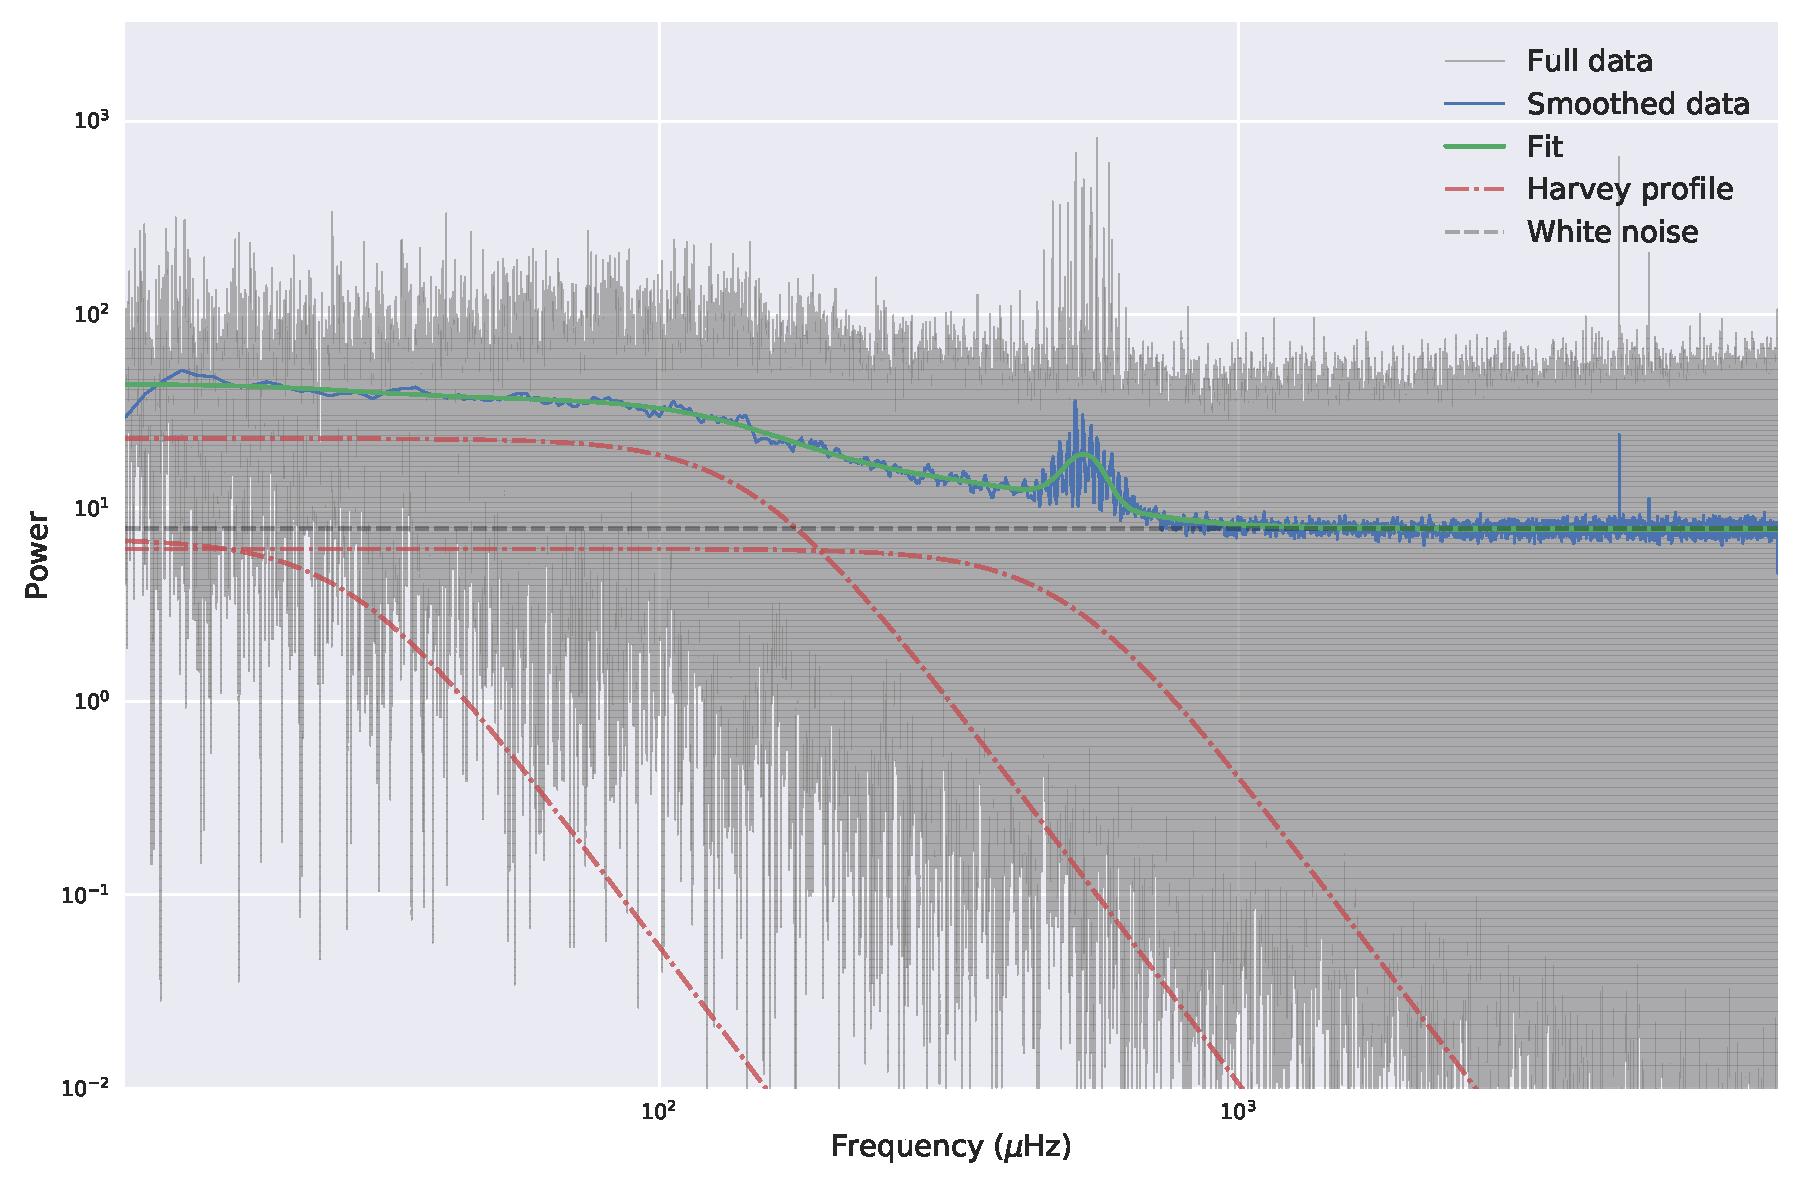
\includegraphics[width=\linewidth]{figs/psd_fit}
			\caption{Results mimicking your figure 1 of my analysis}
		\end{figure}
	
		I won't dwell too much on the differences because I did my analysis in Pymc3 as opposed to Diamonds and I have no information on the priors you used. Some of the big differences are the Harvey profile components. I also had a difference in some of the Gaussian envelope parameters. Again, more discussion on the priors would help with this. 
		
		As for the mode fitting, again I would like to see descriptions of priors. I also would like to see some discussion about how the 32 modes were chosen, initially. Describing how you use the Gaussian envelope from the previous fit to find the range and determine generally where the modes are. I also want to note that consideration needs to be made for asymmetry in oscillation modes that cannot be modeled with a Lorentzian distribution. Finally, at the end of the section, I want to know why a Gaussian was chosen to fit $\nu_{max}$ for each star as opposed to a Lorentzian for every other peak. My results for fitting one peak from the envelope data set is as follows
		
		$$ A \sim N(20, \sigma=10) $$
		$$ \nu_0 \sim N(477, \sigma=2) $$
		$$ L \sim half-Cauchy(\beta=5) $$
		
		\begin{figure}
			\centering
			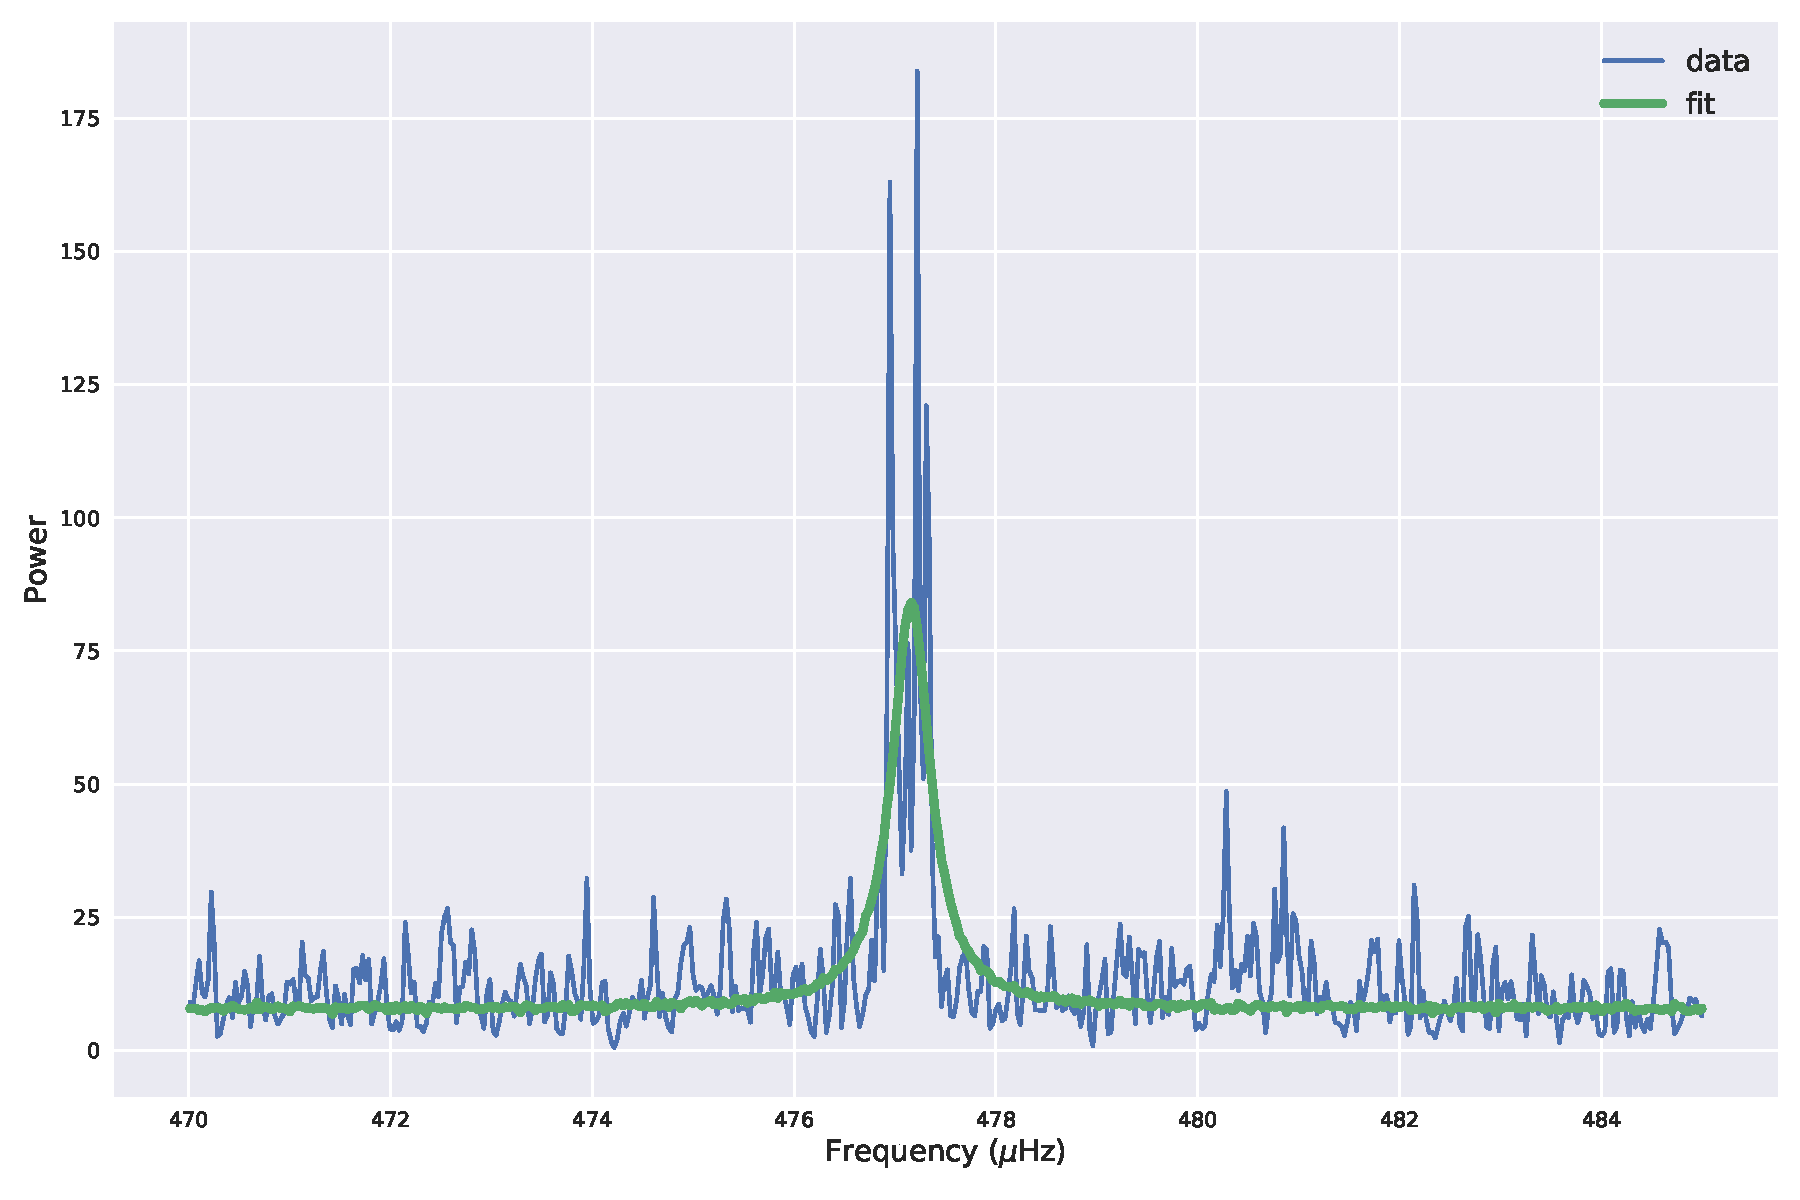
\includegraphics[width=\linewidth]{figs/mode_fit}
			\caption{Results mimicking your figure 2 of my analysis restricted to one peak of interest to reduce dimensionality of sampling.}
		\end{figure}
		
		\section{Asteroseismic Analysis}
		
		I think some clarification needs to be made in section 4.2 paragraph 4. Are $\nu_{obs}$ from your mode fits from the bayesian analysis or from the raw data? Also, at the end of that paragraph, I would like you to describe what too large of a $\chi^2$ value would be for this application. I was able to recreate the grid fitting using MESA models but did not allow myself enough time to ensure their finish, so I cannot comment on the accuracy of that fitting. 
		
		\section{Final Comments}
		
		This is a very nice paper that is pushing the boundaries of astronomy as a science. The major flaws I see are the lack of prior descriptions for your parameters. I also would like to see some more discussion about the echelle diagrams and what you interpret from them, what curving, etc. you see. As this field continues to improve this will be a paper others reference and build upon. Hopefully there is a way to more efficiently model the peaks; the multimodality and high dimensionality is extremely inefficient for sampling with non-specialty code. Hopefully, too, there will come a point where we will not have to resort to evolutionary models for the $l=1$ modes.
		
\end{document}